% Options for packages loaded elsewhere
\PassOptionsToPackage{unicode}{hyperref}
\PassOptionsToPackage{hyphens}{url}
%
\documentclass[
  english,
  man,floatsintext]{apa6}
\usepackage{lmodern}
\usepackage{amssymb,amsmath}
\usepackage{ifxetex,ifluatex}
\ifnum 0\ifxetex 1\fi\ifluatex 1\fi=0 % if pdftex
  \usepackage[T1]{fontenc}
  \usepackage[utf8]{inputenc}
  \usepackage{textcomp} % provide euro and other symbols
\else % if luatex or xetex
  \usepackage{unicode-math}
  \defaultfontfeatures{Scale=MatchLowercase}
  \defaultfontfeatures[\rmfamily]{Ligatures=TeX,Scale=1}
\fi
% Use upquote if available, for straight quotes in verbatim environments
\IfFileExists{upquote.sty}{\usepackage{upquote}}{}
\IfFileExists{microtype.sty}{% use microtype if available
  \usepackage[]{microtype}
  \UseMicrotypeSet[protrusion]{basicmath} % disable protrusion for tt fonts
}{}
\makeatletter
\@ifundefined{KOMAClassName}{% if non-KOMA class
  \IfFileExists{parskip.sty}{%
    \usepackage{parskip}
  }{% else
    \setlength{\parindent}{0pt}
    \setlength{\parskip}{6pt plus 2pt minus 1pt}}
}{% if KOMA class
  \KOMAoptions{parskip=half}}
\makeatother
\usepackage{xcolor}
\IfFileExists{xurl.sty}{\usepackage{xurl}}{} % add URL line breaks if available
\IfFileExists{bookmark.sty}{\usepackage{bookmark}}{\usepackage{hyperref}}
\hypersetup{
  pdftitle={Exploring reliability heterogeneity with multiverse analyses: Data processing decisions unpredictably influence measurement reliability},
  pdfkeywords={reliability, multiverse, analytic flexibility, data processing},
  hidelinks,
  pdfcreator={LaTeX via pandoc}}
\urlstyle{same} % disable monospaced font for URLs
\usepackage{color}
\usepackage{fancyvrb}
\newcommand{\VerbBar}{|}
\newcommand{\VERB}{\Verb[commandchars=\\\{\}]}
\DefineVerbatimEnvironment{Highlighting}{Verbatim}{commandchars=\\\{\}}
% Add ',fontsize=\small' for more characters per line
\usepackage{framed}
\definecolor{shadecolor}{RGB}{248,248,248}
\newenvironment{Shaded}{\begin{snugshade}}{\end{snugshade}}
\newcommand{\AlertTok}[1]{\textcolor[rgb]{0.94,0.16,0.16}{#1}}
\newcommand{\AnnotationTok}[1]{\textcolor[rgb]{0.56,0.35,0.01}{\textbf{\textit{#1}}}}
\newcommand{\AttributeTok}[1]{\textcolor[rgb]{0.77,0.63,0.00}{#1}}
\newcommand{\BaseNTok}[1]{\textcolor[rgb]{0.00,0.00,0.81}{#1}}
\newcommand{\BuiltInTok}[1]{#1}
\newcommand{\CharTok}[1]{\textcolor[rgb]{0.31,0.60,0.02}{#1}}
\newcommand{\CommentTok}[1]{\textcolor[rgb]{0.56,0.35,0.01}{\textit{#1}}}
\newcommand{\CommentVarTok}[1]{\textcolor[rgb]{0.56,0.35,0.01}{\textbf{\textit{#1}}}}
\newcommand{\ConstantTok}[1]{\textcolor[rgb]{0.00,0.00,0.00}{#1}}
\newcommand{\ControlFlowTok}[1]{\textcolor[rgb]{0.13,0.29,0.53}{\textbf{#1}}}
\newcommand{\DataTypeTok}[1]{\textcolor[rgb]{0.13,0.29,0.53}{#1}}
\newcommand{\DecValTok}[1]{\textcolor[rgb]{0.00,0.00,0.81}{#1}}
\newcommand{\DocumentationTok}[1]{\textcolor[rgb]{0.56,0.35,0.01}{\textbf{\textit{#1}}}}
\newcommand{\ErrorTok}[1]{\textcolor[rgb]{0.64,0.00,0.00}{\textbf{#1}}}
\newcommand{\ExtensionTok}[1]{#1}
\newcommand{\FloatTok}[1]{\textcolor[rgb]{0.00,0.00,0.81}{#1}}
\newcommand{\FunctionTok}[1]{\textcolor[rgb]{0.00,0.00,0.00}{#1}}
\newcommand{\ImportTok}[1]{#1}
\newcommand{\InformationTok}[1]{\textcolor[rgb]{0.56,0.35,0.01}{\textbf{\textit{#1}}}}
\newcommand{\KeywordTok}[1]{\textcolor[rgb]{0.13,0.29,0.53}{\textbf{#1}}}
\newcommand{\NormalTok}[1]{#1}
\newcommand{\OperatorTok}[1]{\textcolor[rgb]{0.81,0.36,0.00}{\textbf{#1}}}
\newcommand{\OtherTok}[1]{\textcolor[rgb]{0.56,0.35,0.01}{#1}}
\newcommand{\PreprocessorTok}[1]{\textcolor[rgb]{0.56,0.35,0.01}{\textit{#1}}}
\newcommand{\RegionMarkerTok}[1]{#1}
\newcommand{\SpecialCharTok}[1]{\textcolor[rgb]{0.00,0.00,0.00}{#1}}
\newcommand{\SpecialStringTok}[1]{\textcolor[rgb]{0.31,0.60,0.02}{#1}}
\newcommand{\StringTok}[1]{\textcolor[rgb]{0.31,0.60,0.02}{#1}}
\newcommand{\VariableTok}[1]{\textcolor[rgb]{0.00,0.00,0.00}{#1}}
\newcommand{\VerbatimStringTok}[1]{\textcolor[rgb]{0.31,0.60,0.02}{#1}}
\newcommand{\WarningTok}[1]{\textcolor[rgb]{0.56,0.35,0.01}{\textbf{\textit{#1}}}}
\usepackage{graphicx,grffile}
\makeatletter
\def\maxwidth{\ifdim\Gin@nat@width>\linewidth\linewidth\else\Gin@nat@width\fi}
\def\maxheight{\ifdim\Gin@nat@height>\textheight\textheight\else\Gin@nat@height\fi}
\makeatother
% Scale images if necessary, so that they will not overflow the page
% margins by default, and it is still possible to overwrite the defaults
% using explicit options in \includegraphics[width, height, ...]{}
\setkeys{Gin}{width=\maxwidth,height=\maxheight,keepaspectratio}
% Set default figure placement to htbp
\makeatletter
\def\fps@figure{htbp}
\makeatother
\setlength{\emergencystretch}{3em} % prevent overfull lines
\providecommand{\tightlist}{%
  \setlength{\itemsep}{0pt}\setlength{\parskip}{0pt}}
\setcounter{secnumdepth}{-\maxdimen} % remove section numbering
% Make \paragraph and \subparagraph free-standing
\ifx\paragraph\undefined\else
  \let\oldparagraph\paragraph
  \renewcommand{\paragraph}[1]{\oldparagraph{#1}\mbox{}}
\fi
\ifx\subparagraph\undefined\else
  \let\oldsubparagraph\subparagraph
  \renewcommand{\subparagraph}[1]{\oldsubparagraph{#1}\mbox{}}
\fi
% Manuscript styling
\usepackage{upgreek}
\captionsetup{font=singlespacing,justification=justified}

% Table formatting
\usepackage{longtable}
\usepackage{lscape}
% \usepackage[counterclockwise]{rotating}   % Landscape page setup for large tables
\usepackage{multirow}		% Table styling
\usepackage{tabularx}		% Control Column width
\usepackage[flushleft]{threeparttable}	% Allows for three part tables with a specified notes section
\usepackage{threeparttablex}            % Lets threeparttable work with longtable

% Create new environments so endfloat can handle them
% \newenvironment{ltable}
%   {\begin{landscape}\begin{center}\begin{threeparttable}}
%   {\end{threeparttable}\end{center}\end{landscape}}
\newenvironment{lltable}{\begin{landscape}\begin{center}\begin{ThreePartTable}}{\end{ThreePartTable}\end{center}\end{landscape}}

% Enables adjusting longtable caption width to table width
% Solution found at http://golatex.de/longtable-mit-caption-so-breit-wie-die-tabelle-t15767.html
\makeatletter
\newcommand\LastLTentrywidth{1em}
\newlength\longtablewidth
\setlength{\longtablewidth}{1in}
\newcommand{\getlongtablewidth}{\begingroup \ifcsname LT@\roman{LT@tables}\endcsname \global\longtablewidth=0pt \renewcommand{\LT@entry}[2]{\global\advance\longtablewidth by ##2\relax\gdef\LastLTentrywidth{##2}}\@nameuse{LT@\roman{LT@tables}} \fi \endgroup}

% \setlength{\parindent}{0.5in}
% \setlength{\parskip}{0pt plus 0pt minus 0pt}

% \usepackage{etoolbox}
\makeatletter
\patchcmd{\HyOrg@maketitle}
  {\section{\normalfont\normalsize\abstractname}}
  {\section*{\normalfont\normalsize\abstractname}}
  {}{\typeout{Failed to patch abstract.}}
\makeatother
\shorttitle{Reliability multiverse}
\author{Sam Parsons\textsuperscript{1}}
\affiliation{
\vspace{0.5cm}
\textsuperscript{1} University of Oxford}
\authornote{Submitted to Meta-Psychology. Click here to follow the fully transparent editorial process of this submission. Participate in open peer review by commenting through hypothes.is directly on this preprint.

This work was supported by an ESRC grant [ES/R004285/1]

I would like to thank Ana Todorovic for her insightful feedback on an earlier version of this manuscript.


Correspondence concerning this article should be addressed to Sam Parsons, Department of Experimental Psychology, University of Oxford, New Radcliffe House, Radcliffe Observatory Quarter, Oxford, OX2 6AE. E-mail: sam.parsons@psy.ox.ac.uk}
\keywords{reliability, multiverse, analytic flexibility, data processing}
\usepackage{csquotes}
\usepackage{float}
\usepackage{caption}
\usepackage{newunicodechar}
\floatplacement{figure}{H}
\raggedbottom
\ifxetex
  % Load polyglossia as late as possible: uses bidi with RTL langages (e.g. Hebrew, Arabic)
  \usepackage{polyglossia}
  \setmainlanguage[]{english}
\else
  \usepackage[shorthands=off,main=english]{babel}
\fi

\title{Exploring reliability heterogeneity with multiverse analyses: Data processing decisions unpredictably influence measurement reliability}

\date{}

\abstract{
Analytic flexibility is known to influence the results of statistical tests, e.g.~effect sizes and \emph{p}-values. Yet, the degree to which flexibility in data-processing decisions influences the reliability of our measures is unknown. In this paper I attempt to address this question using a series of reliability multiverse analyses. The methods section incorporates a brief tutorial for readers interested in implementing multiverse analyses reported in this manuscript; all functions are contained in the R package \emph{splithalf}. I report six multiverse analyses of data-processing specifications, including accuracy and response time cutoffs. I used data from a Stroop task and Flanker task at two time points. This allowed for an internal consistency reliability multiverse at time 1 and 2, and a test-retest reliability multiverse between time 1 and 2. Largely arbitrary decisions in data-processing led to differences between the highest and lowest reliability estimate of at least 0.2. Importantly, there was no consistent pattern in the data-processing specifications that led to greater reliability, across time as well as tasks. Together, data-processing decisions are highly influential, and largely unpredictable, on measure reliability. I discuss actions researchers could take to mitigate some of the influence of reliability heterogeneity, including adopting hierarchical modelling approaches. Yet, there are no approaches that can completely save us from measurement error. Measurement matters and I call on readers to help us move from what could be a measurement crisis towards a measurement revolution.
}

\begin{document}
\maketitle

The vermilisitude of our conclusions rests on the quality, and the strength, of our evidence. Our evidence rests on the bedrock of our measurements. The quality of our measures defines the quality of our results. Without adequate focus on the validity of our measures, how can we be assured that we are capturing the concept or process that we are interested in? Without any attention to the reliability of our measures, how can we be sure that we are capturing a phenomenon with any precision? Psychological science -- I concede some areas are better than others - has a guilty habit of neglecting these foundations.

In a recent paper, my colleagues and I argued for a widespread appreciation for the reliability of our cognitive measures (Parsons et al., 2019). Briefly; low reliability places doubt on the veracity of statistical analyses using that measure; measurement reliability restricts the observable range of effect sizes; and failing to correct for measurement error makes comparing effect sizes between, and within, studies difficult. These issues are compounded by the sad observation that the reporting of reliability (and validity) evidence is woefully poor. Scale validity and reliability is not routinely examined, and many scales are adapted on an ad hoc basis with little or no validation (Flake, Pek, \& Hehman, 2017). In other cases scales fail to pass deeper psychometric evaluation, including tests of measurement invariance (Hussey \& Hughes, 2018). This likely reflects issues with more superficial approaches to establishing validity evidence - i.e.~reporting Cronbach's alpha, stating it is adequate, and moving on. I concede that pockets of psychological science take a more enlightened approach. However, I feel it is reasonable to argue that the field at large is doing well in our measurement practices. Most relevant to this paper; it is the exception rather than the norm to evaluate the psychometric properties of cognitive measurements (Gawronski, Deutsch, \& Banse, 2011).

An important reminder: estimates of reliability refer to the measurement obtained - in a specific sample and under particular circumstances, including the task parameters. Reliability is therefore not fixed; it may differ between populations, samples, and testing conditions. Variations of a task may lead to the generation of more or less reliable measurements. For example, the stimulus presentation duration will likely influence the cognitive processes involved in completing the task, perhaps leading participants to perform more consistently in one version, relative to another. Reliability is a property of the measurement, not of the task used to obtain it. Strictly speaking, we cannot state that a task is unreliable; although we might observe a consistent pattern of unreliability in measurements obtained that causes us to question further use of the task.

Thankfully, there is a growing awareness that measurement matters (Fried \& Flake, 2018). A valuable term, Questionable Measurement Practices (QMPs), was recently added to our vernacular by Flake and Fried (2019). QMPs describe \enquote{undisclosed decisions researchers make that leave questions about the measurements in a study unanswered} (page 2). I hope that QMPs and the importance of measurement become as widely discussed as the parallel idiom, \enquote{Questionable Research Practices} (QRPs). Most importantly, wider discussion of these practices should make it clear to all researchers that we make many potentially impactful decisions in the design of our measures, our data processing or cleaning, and our data analysis.

In this paper I was concerned with the influence analytic flexibility on measurement reliability, specifically in data processing or data cleaning. I was inspired in part from numerous papers reporting the unsettlingly low reliability of dot-probe attention bias indices (e.g.~Jones, Christiansen, \& Field, 2018; Schmukle, 2005; Staugaard, 2009). I was also inspired by other work investigating alternative analyses and data processing strategies, with the intention of yielding a more reliable measurement (e.g.~Jones et al., 2018; Price et al., 2015). I was interested in visualising the influence of data processing steps on reliability. My rationale was that as all too often the focus is on decisions made in the beginning (task design) or at the end (data analysis) of the research process. I felt the intermediary stage in which the data is processed is often unexplored in relation to QRPs and QMPs. To fully explain my rationale, we first take a walk through the garden of forking paths.

\hypertarget{analytic-flexibility-and-the-garden-of-forking-paths}{%
\subsection{Analytic flexibility and the garden of forking paths}\label{analytic-flexibility-and-the-garden-of-forking-paths}}

Every result presented in every research article is the culmination of many decisions made by one or more researchers; the sheer number of combinations of valid decisions is likely uncalculatable. The \enquote{garden of forking paths} (Gelman \& Loken, 2013) is a useful analogy I use throughout this paper to illustrate this. With each decision that must be made, however arbitrary, the researcher comes to a fork in their research path, and selects one. To add a little suspense, there will be many cases when the researcher does not notice a fork in the road. Perhaps the researcher unconsciously makes the same turn as always, their feet working of their own accord. These forks in the path, the decisions researchers make (whether they are aware or not), may be reasonably combined to make a near uncountable number of paths. Each path also leads to a location; some paths end close to one another, and other times the paths diverge wildly. We can think of the end of the path as the statistical result our researcher arrives at.

The researcher has to decide their path, based on the soundest justifications they can make at each fork (e.g.~Lakens et al., 2018). Of course, psychological science has become fully aware of the detrimental effects of selecting one's path retrospectively, based on where the path ends or the results most exciting to the researcher (read as: \emph{p} \textless{} .05; e.g.~Simmons, Nelson, \& Simonsohn, 2011). Extending the metaphor (hopefully not too painfully): Backtracking the route and selecting multiple paths until reaching a preferred location is akin to walking between the well-tended paths and stomping across the flowerbeds, damaging our colourful science garden. Analytic flexibility is not inherently bad. However, we must acknowledge the ramifications. The effects we observe, or do not, are potentially influenced by all of the decisions made to arrive at them. Thus, a range of possible effects may have been observed that are all equally valid based on the analytical decisions made.

In discussions of analytical flexibility, focus is usually given primarily to decisions made during statistical analysis. For example; should I control for age and gender? Do I reason that this is model more appropriate over that one? Or, where should I set my alpha and how should I justify the decision? Discussions of analytical flexibility often concern issues around \emph{p}-hacking and other QRPs (intended or unintended). However, as Leek and Peng (2015) note, \emph{p}-values are the tip of the iceberg; not enough scrutiny is given to the impact of the many steps in the research pipeline that precede inference testing. I agree. In my estimation, flexibility in measurement and data handling do not receive the scrutiny they deserve. If the garden of forking paths concerns analytic flexibility, then measurement flexibility decides which door one enters the garden through in the first place.

\hypertarget{mapping-the-garden-of-forking-paths-with-multiverse-analyses}{%
\subsection{Mapping the garden of forking paths with multiverse analyses}\label{mapping-the-garden-of-forking-paths-with-multiverse-analyses}}

A multiverse analysis (Steegen, Tuerlinckx, Gelman, \& Vanpaemel, 2016) offers us a \enquote{GPS in the garden of forking paths} (Quintana \& Heathers, 2019). The process is remarkably simple. First, we define a set of reasonable data processing and analysis decisions. Second, we run the entire set of analyses. We can then examine results across the entire range of results. Specification curve analysis (Simonsohn, Simmons, \& Nelson, 2015) adds third step allowing for inference tests across the distribution of results generated in the multiverse (for insightful applications of specification curve analyses, see; Orben \& Przybylski, 2019; Rohrer, Egloff, \& Schmukle, 2017). In this paper I use \enquote{specification} to refer to each combination of data processing decisions in the multiverse analysis.

Multiverse analyses enable us to explore how a researcher's -- sometimes arbitrary -- choices in data processing (e.g.~outlier removal) and analysis decisions (e.g.~including covariates, splitting samples) influence statistical results, and the conclusions drawn from the analysis. From this we can examine which choices are more or less influential than others, as well as how robust the result is across the full set of specifications.

\hypertarget{a-reliability-multiverse-from-many-data-processing-decisions}{%
\subsection{A reliability multiverse from many data processing decisions}\label{a-reliability-multiverse-from-many-data-processing-decisions}}

In this paper I report multiverse analyses exploring the influence of data processing specifications on the reliability of a calculated measurement. I used openly accessible Stroop task and Flanker task data generously shared by Hedge and colleagues (Hedge, Powell, \& Sumner, 2018). Following previous work in this area (Parsons et al., 2019), I was interested in the stability and range of reliability estimates on cognitive-behavioural measures. Broadly, I was interested in the positive and negative impact of data processing decisions on reliability. It is possible that certain analytic decisions tend to yield higher reliability estimates; it may be that particular combinations of decisions are also better, or worse, than others. Beyond that, I was interested in the range of estimates. A small range would suggest that measure reliability is relatively stable as we make potentially arbitrary data processing decisions while walking the garden of forking paths. A large range suggests hidden measurement reliability heterogeneity. This is potentially an important, and underappreciated, contributor to the replicability crisis (Loken \& Gelman, 2017). Alternatively, this could be a herald for a crisis of measurement.

\hypertarget{methods}{%
\section{Methods}\label{methods}}

\hypertarget{data}{%
\subsection{Data}\label{data}}

Data were obtained from the online repository for Hedge, Sumner, and Powell ((2018); \url{https://osf.io/cwzds/}). Full details of the data collection, study design, and procedure can be found in Hedge et al.~(2018). These data are ideal for our purposes as they a) contain many trials, helping us obtain more precise estimates of reliability, and b) include two assessment time-points approximately 3-4 weeks apart, allowing us to explore both; internal consistency and test-retest reliability. The data were collected from different studies; for simplicity in this paper, the data across studies were pooled (n = 107 before any data processing -- note that this may be different from the sample size presented by Hedge et al.~due to differences in data processing). I explored data from the Stroop and the Flanker tasks. Interested readers can find the data and code used to perform the multiverse analyses and generate this manuscript in the Open Science Framework repository for this project (\url{https://osf.io/haz6u/}).\footnote{I used the following R packages for all analyses and figures, and to generate this document: R (Version 3.6.3; R Core Team, 2018) and the R-packages \emph{Cairo} (Version 1.5.12; Urbanek \& Horner, 2019), \emph{dplyr} (Version 0.8.5; Wickham et al., 2019), \emph{forcats} (Version 0.5.0; Wickham, 2019a), \emph{ggplot2} (Version 3.3.0; Wickham, 2016), \emph{gridExtra} (Version 2.3; Auguie, 2017), \emph{papaja} (Version 0.1.0.9942; Aust \& Barth, 2020), \emph{patchwork} (Version 1.0.0; Pedersen, 2019), \emph{psych} (Version 1.9.12.31; Revelle, 2019), \emph{purrr} (Version 0.3.4; Henry \& Wickham, 2019), \emph{readr} (Version 1.3.1; Wickham, Hester, \& Francois, 2018), \emph{splithalf} (Version 0.7.1; Parsons, 2020), \emph{stringr} (Version 1.4.0; Wickham, 2019b), \emph{tibble} (Version 3.0.1; Müller \& Wickham, 2019), \emph{tidyr} (Version 1.1.0; Wickham \& Henry, 2019), and \emph{tidyverse} (Version 1.3.0; Wickham, Averick, et al., 2019)}

\hypertarget{stroop-task}{%
\subsubsection{Stroop task}\label{stroop-task}}

Participants made keyed responses to the colour of a word presented in the centre of the screen. In congruent conditions the word was the same as the font colour, whereas, in incongruent trials, the word was a different colour from the font colour. In a neutral condition, the word was not a colour word. Participants completed 240 of each trial type. The outcome index we explore here is the RT cost, calculated as the average RT for incongruent trials minus the average RT for congruent trials.

\hypertarget{flanker-task}{%
\subsubsection{Flanker task}\label{flanker-task}}

Participants made keyed responses to the direction of an arrow presented in the centre of the screen. The central arrow was flanked by two other symbols. Congruent trials presented flanking arrows in the same direction as the central arrow, whereas incongruent trials presented flanking arrows in the opposite direction to the central arrow. There was also a neutral condition in which flanking symbols were straight lines. Participants completed 240 of each trial type. The outcome index we explore here is the RT cost, calculated as the average RT for incongruent trials minus the average RT for congruent trials.

\hypertarget{multiverse-analysis}{%
\subsection{Multiverse analysis}\label{multiverse-analysis}}

In a personal effort to make my research reproducible, and also help others perform similar processes I have developed simple functions to perform the multiverse analyses reported in this paper. The key functions are: \emph{splithalf.multiverse}, \emph{testretest.multiverse}, and \emph{multiverse.plot}. These functions appear in the the \emph{splithalf} package (Parsons (2019); starting at version 0.7.1) and are also provided separately in the supplemental materials.

The functions use R packages \emph{splithalf} (Parsons, 2019) and \emph{psych} (Revelle, 2017) to estimate internal consistency and test-retest reliability, respectively. Moreover, this section acts as a brief tutorial with the aim of helping interested readers conduct their own reliability multiverse analysis with different data or sets of specifications (also see full code: \url{https://osf.io/haz6u/}).

\hypertarget{step-1.-creating-a-list-of-all-specifications}{%
\subsubsection{Step 1. Creating a list of all specifications}\label{step-1.-creating-a-list-of-all-specifications}}

No data were removed before the multiverse analysis. To my knowledge, there are no fixed standards in the literature for processing Stroop or Flanker data. I identified six decisions common to processing RT data, though there are many more. For simplicity I stuck to RT difference scores as the outcome measure of interest. However, there are very different analytical techniques that might be applied to RT tasks such as this (for example, multilevel modelling and drift-diffusion modelling approaches). The decisions were as follows:

\begin{itemize}
\item
  \emph{Total accuracy.} Researchers may opt to remove participants with accuracy lower than a pre-specified cut-off; for example 80 of 90 per cent. I used three options; 80\%, 90\%, and no cut-off.
\item
  \emph{Absolute response time removals.} Researchers will often remove trials faster than a minimum RT threshold and trials that exceed a maximum RT threshold. I use minimum RT cut-offs at 100ms, 200ms, as well as no cut-off. And, I use two maximum RT cutoffs; 3000ms, and 2000ms.
\item
  \emph{Relative RT cut offs.} After absolute RT cut-offs, researchers can decide to remove trials with RTs greater than a number of standard deviations from the mean (sometimes called relative cut-offs or trimmed means). Three SDs from the mean would remove very extreme outliers; two SDs from the mean is common. I have not seen researchers use one SD from the mean as a cut off, as it is likely a too conservative threshold. As I was interested in a wide range of possible specifications, I included one standard deviation. I use no relative cut off, and one, two, and three SDs from the mean cutoffs in the multiverse.
\item
  \emph{Where to apply the relative cutoff.} The decision to remove trials based on a SD cutoff comes with its own decision. Namely, at what granularity? We could remove trials with RTs greater than 2SDs from the participant's average RT, for example. We could also remove trials with RTs greater than 2SDs from the mean RT within each trial type (congruent and incongruent, for example). I included both options; participant level, and trial type level.
\item
  \emph{Averaging.} Most often the mean RT within each trial type is calculated, and may then be analysed directly, or a difference score calculated to analyse. Researchers may opt to use the median RT instead. I included both options.
\end{itemize}

The number of possible combinations (data processing specifications) quickly increases with every additional option. Here we have 3 \(\times\) 2 \(\times\) 3 \(\times\) 4 \(\times\) 2 \(\times\) 2 = 288 possible specifications. We can specify our list of decisions as follows:

\begin{Shaded}
\begin{Highlighting}[]
\NormalTok{specifications <-}\StringTok{ }\KeywordTok{list}\NormalTok{(}
 \DataTypeTok{ACC_cutoff =} \KeywordTok{c}\NormalTok{(}\DecValTok{0}\NormalTok{, }\FloatTok{0.8}\NormalTok{, }\FloatTok{0.9}\NormalTok{),  }
 \DataTypeTok{RT_min           =} \KeywordTok{c}\NormalTok{(}\DecValTok{0}\NormalTok{, }\DecValTok{100}\NormalTok{, }\DecValTok{200}\NormalTok{),}
 \DataTypeTok{RT_max            =} \KeywordTok{c}\NormalTok{(}\DecValTok{2000}\NormalTok{, }\DecValTok{3000}\NormalTok{),}
 \DataTypeTok{RT_sd_cutoff      =} \KeywordTok{c}\NormalTok{(}\DecValTok{0}\NormalTok{, }\DecValTok{1}\NormalTok{, }\DecValTok{2}\NormalTok{, }\DecValTok{3}\NormalTok{),}
 \DataTypeTok{split_by          =} \KeywordTok{c}\NormalTok{(}\StringTok{"subject"}\NormalTok{, }\StringTok{"trial"}\NormalTok{), }
 \DataTypeTok{averaging_method  =} \KeywordTok{c}\NormalTok{(}\StringTok{"mean"}\NormalTok{, }\StringTok{"median"}\NormalTok{)}
\NormalTok{)}
\end{Highlighting}
\end{Shaded}

\hypertarget{step-2.-run-all-specifications-and-extract-reliability-estimates}{%
\subsubsection{Step 2. Run all specifications and extract reliability estimates}\label{step-2.-run-all-specifications-and-extract-reliability-estimates}}

From this decision list, we have a complete list of 288 data processing specifications. In the multiverse analysis the data is processed following each specification parameters, before estimating the reliability of the resulting outcome measure. In the following example code we perform a multiverse analysis on the Stroop data from Hedge et al.'s first testing session. First, we run \emph{splithalf} on the full dataset and save the output into a splithalf object.\footnote{Note that if users want to run a multiverse on multiple task conditions (e.g.~happy and sad stimuli, or time 1 and time 2) they must specify separate multiverse analyses} We then pass this object into \emph{splithalf.multiverse.} The only required inputs are the specification list, and our saved splithalf object.

\begin{Shaded}
\begin{Highlighting}[]
\NormalTok{splithalf_}\DecValTok{1}\NormalTok{ <-}\StringTok{ }\KeywordTok{splithalf}\NormalTok{(}\DataTypeTok{data =} \KeywordTok{subset}\NormalTok{(Hedge_raw_Stroop, time }\OperatorTok{==}\StringTok{ }\DecValTok{1}\NormalTok{),}
                         \DataTypeTok{permutations =} \DecValTok{500}\NormalTok{,}
                         \DataTypeTok{var.ACC =} \StringTok{"Correct"}\NormalTok{)}

\NormalTok{multiverse_}\DecValTok{1}\NormalTok{ <-}\StringTok{ }\KeywordTok{splithalf.multiverse}\NormalTok{(}\DataTypeTok{input =}\NormalTok{ splithalf_}\DecValTok{1}\NormalTok{,}
                 \DataTypeTok{specifications =}\NormalTok{ specifications)}
\end{Highlighting}
\end{Shaded}

The output contains useful information, including; the data, the expanded specification list, each processed dataset, and information about the call. Most important is the \enquote{estimates} data frame, which contains the reliability estimate for each specification. The \enquote{removals} list can be used to inspect the number of participants and trials remaining following data reduction. \enquote{CI} can be used to inspect the median and 95\% CI of all reliability estimates.

\hypertarget{step-3.-visualising-the-multiverse}{%
\subsubsection{Step 3. Visualising the multiverse}\label{step-3.-visualising-the-multiverse}}

I find that one of the joys of multiverse analyses are the visualisations; because sometimes science is more art than science. The results section is centred on these visualisations. We use the output from \emph{splithalf.multiverse} in the function multiverse.plot to visualise the specification curve of reliability estimates. It can be called with the following;

\begin{Shaded}
\begin{Highlighting}[]
\KeywordTok{multiverse.plot}\NormalTok{(}\DataTypeTok{multiverse =}\NormalTok{ multiverse_}\DecValTok{1}\NormalTok{,}
         \DataTypeTok{title =} \StringTok{"My first multiverse"}\NormalTok{)}
\end{Highlighting}
\end{Shaded}

I explain the visualisations in the results section. I have also added functionality to visualise multiple multiverses in the same plot. To do so, the user can specify a list of multiverse objects. For example:

\begin{Shaded}
\begin{Highlighting}[]
\KeywordTok{multiverse.plot}\NormalTok{(}\DataTypeTok{multiverse =} \KeywordTok{list}\NormalTok{(multiverse_}\DecValTok{1}\NormalTok{,}
\NormalTok{                                  multiverse_}\DecValTok{2}\NormalTok{))}
\end{Highlighting}
\end{Shaded}

\hypertarget{inferences-from-the-multiverse}{%
\subsubsection{Inferences from the multiverse}\label{inferences-from-the-multiverse}}

It is not my aim in this paper to make inferences from these reliability multiverse analyses as one would in a specification curve analysis (Simonsohn et al., 2015). One could use this method to perform inference testing against the curve of reliability estimates. However, it is not clear what this would add: testing whether the reliability estimates significantly differ from zero is a low bar for assessing the reliability of a measure.

Descriptively, it will be useful to explore the full range of estimates. The multiverse objects contain a \enquote{CI} object to help extract the median and 95\% percentile estimates. The user can obtain these by running \texttt{internal.1\_Stroop\$CI}. I have also provided a small function \emph{threshold} to inspect the proportion of reliability estimates above or below a set threshold. Users can specify whether they are interested in the point estimates or the Confidence Intervals. For example, the following will return the proportion of estimates above a 0.7 threshold (often the lowest bar to describe internal consistency estimates as \enquote{acceptable}).

\begin{Shaded}
\begin{Highlighting}[]
\KeywordTok{threshold}\NormalTok{(}\DataTypeTok{multiverse =}\NormalTok{ internal}\FloatTok{.1}\NormalTok{_Stroop,}
          \DataTypeTok{threshold =} \FloatTok{0.7}\NormalTok{,}
          \DataTypeTok{use =} \StringTok{"estimate"}\NormalTok{,}
          \DataTypeTok{dir =} \StringTok{"above"}\NormalTok{)}
\end{Highlighting}
\end{Shaded}

\hypertarget{analysis-plan}{%
\subsection{Analysis plan}\label{analysis-plan}}

In total, I performed six multiverse analyses following the steps described above. Separately for each of the Stroop and Flanker task data, I examined internal consistency reliability at time 1 and at time 2, as well as test-retest reliability from time 1 to time 2. Internal consistency was estimated using 500 permutations of the splithalf procedure for each specification (5000 is standard, but 500 was selected to reduce processing time). For each multiverse I report the median estimate and it's 95\% Confidence Interval, the proportion of estimates exceeding 0.7, and the range of estimates in that multiverse. In addition to visualising each multiverse, I also include visualisations overlapping the internal consistency multiverses from time 1 and time 2. These overlapped plots allow us to visually inspect whether the pattern of reliability estimates following the full range of data processing specifications are comparable across each time point.

\hypertarget{results}{%
\section{Results}\label{results}}

I include a visualisation for each multiverse analysis. The reliability estimates are presented on the y axis at the top of the figure; each estimate is represented by a black dot and the 95\% confidence interval is represented by the shaded band. The x axis indicates each individual multiverse specification of processing decisions (288 total), displayed in the \enquote{dashboard} at the bottom of the figure. The vertical dashed line running through the top panel and the bottom dashboard represents the median reliability estimate. This line is extended through the dashboard to demonstrate that the estimate is derived from the unique combination of data processing decisions, including (from top to bottom, in order of processing step); 1) participant removal below total accuracy threshold, 2) maximum RT cutoff, 3) minimum RT cutoff, 4) removal of RTs \textgreater{} this number of SDs from the mean, 5) whether this removal is at the trial or subject level, and 6) use of mean or median to derive averages.

\newpage

\hypertarget{stroop-time-1-internal-consistency}{%
\subsubsection{Stroop Time 1: Internal Consistency}\label{stroop-time-1-internal-consistency}}

The median reliability estimate was 0.77, 95\% CI {[}0.69,0.91{]}. Estimates ranged from 0.68 to 0.91. 96\% of the reliability estimates were \textgreater{} 0.7.

\begin{figure}
\centering
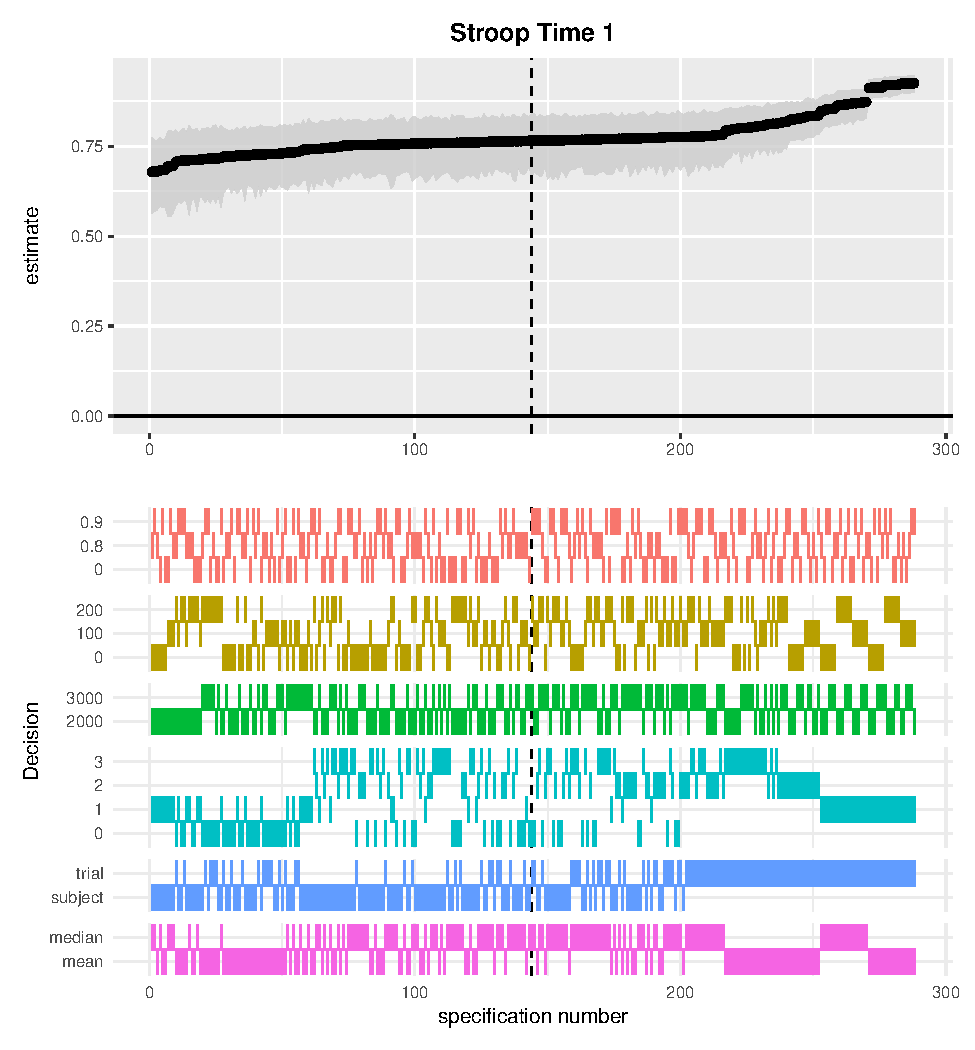
\includegraphics{Reliability_Multiverse_files/figure-latex/unnamed-chunk-5-1.pdf}
\caption{\label{fig:unnamed-chunk-5}Internal consistency reliability multiverse for Stroop RT cost at time 1}
\end{figure}

\newpage

\hypertarget{stroop-time-2-internal-consistency}{%
\subsubsection{Stroop Time 2: Internal Consistency}\label{stroop-time-2-internal-consistency}}

The median reliability estimate was 0.67, 95\% CI {[}0.61,0.88{]}. Estimates ranged from 0.59 to 0.89. 29.00\% of the reliability estimates were \textgreater{} 0.7.

\begin{figure}
\centering
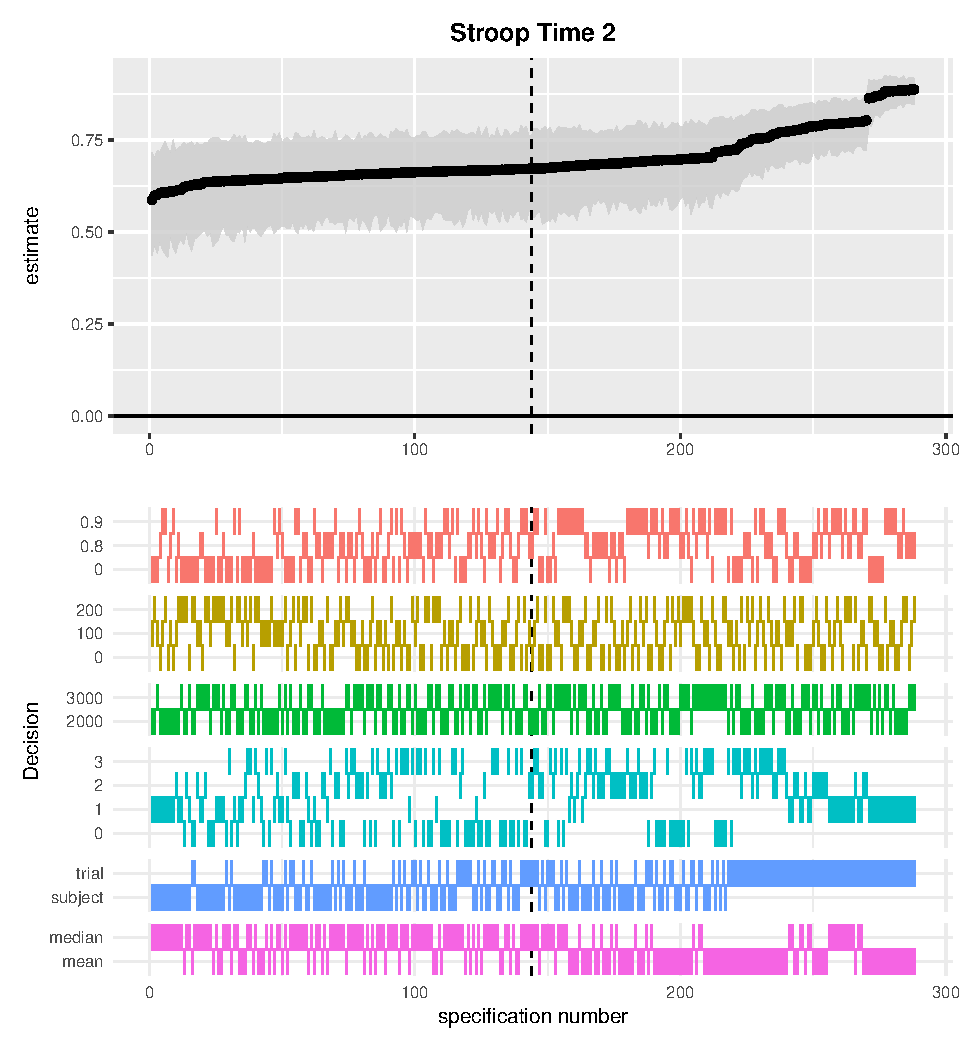
\includegraphics{Reliability_Multiverse_files/figure-latex/unnamed-chunk-6-1.pdf}
\caption{\label{fig:unnamed-chunk-6}Internal consistency reliability multiverse for Stroop RT cost at time 2}
\end{figure}

\newpage

\hypertarget{stroop-test-retest}{%
\subsubsection{Stroop: test-retest}\label{stroop-test-retest}}

The median reliability estimate was 0.56, 95\% CI {[}0.50,0.63{]}. Estimates ranged from 0.47 to 0.63. 0\% of the reliability estimates were \textgreater{} 0.7.

\begin{figure}
\centering
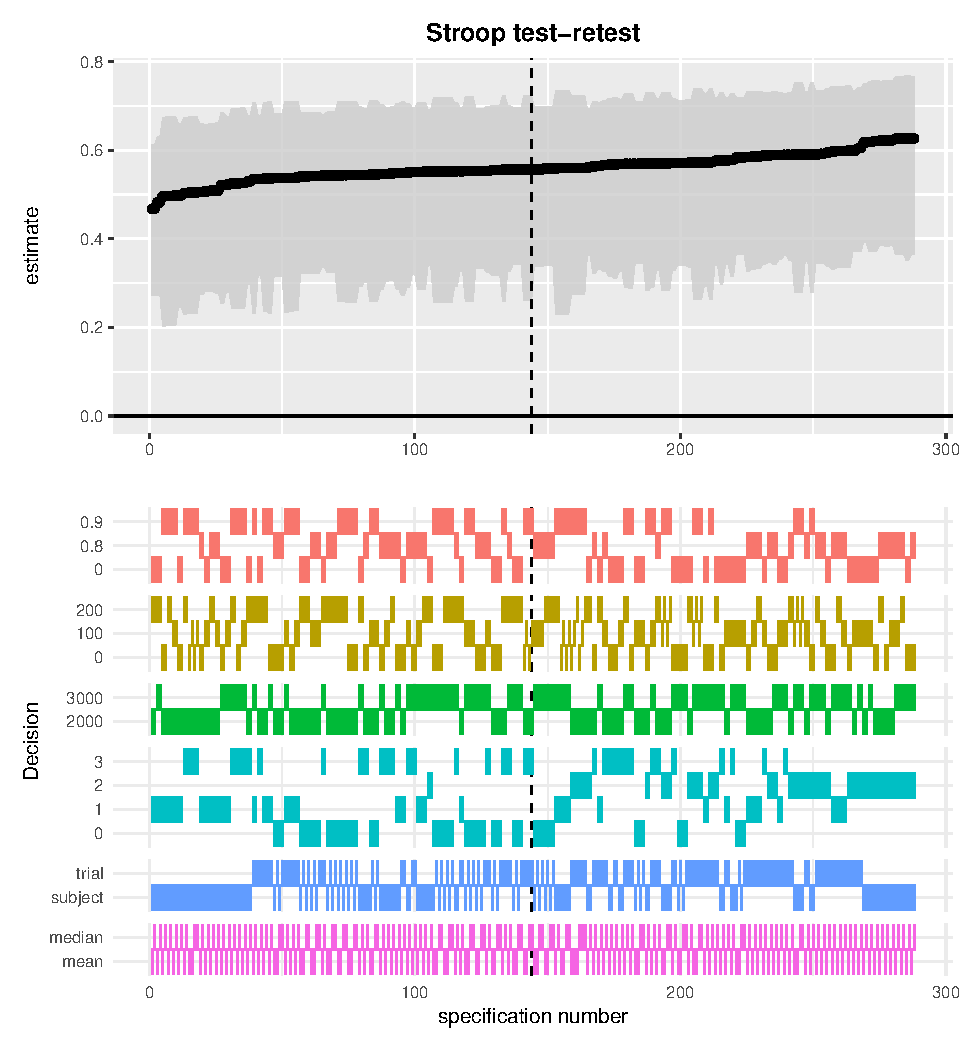
\includegraphics{Reliability_Multiverse_files/figure-latex/unnamed-chunk-7-1.pdf}
\caption{\label{fig:unnamed-chunk-7}Test-retest reliability multiverse for Stroop RT cost}
\end{figure}

\newpage

\hypertarget{flanker-time-1-internal-consistency}{%
\subsubsection{Flanker Time 1: Internal Consistency}\label{flanker-time-1-internal-consistency}}

The median reliability estimate was 0.84, 95\% CI {[}0.70,0.92{]}. Estimates ranged from 0.63 to 0.93. 98\% of the reliability estimates were \textgreater{} 0.7.

\begin{figure}
\centering
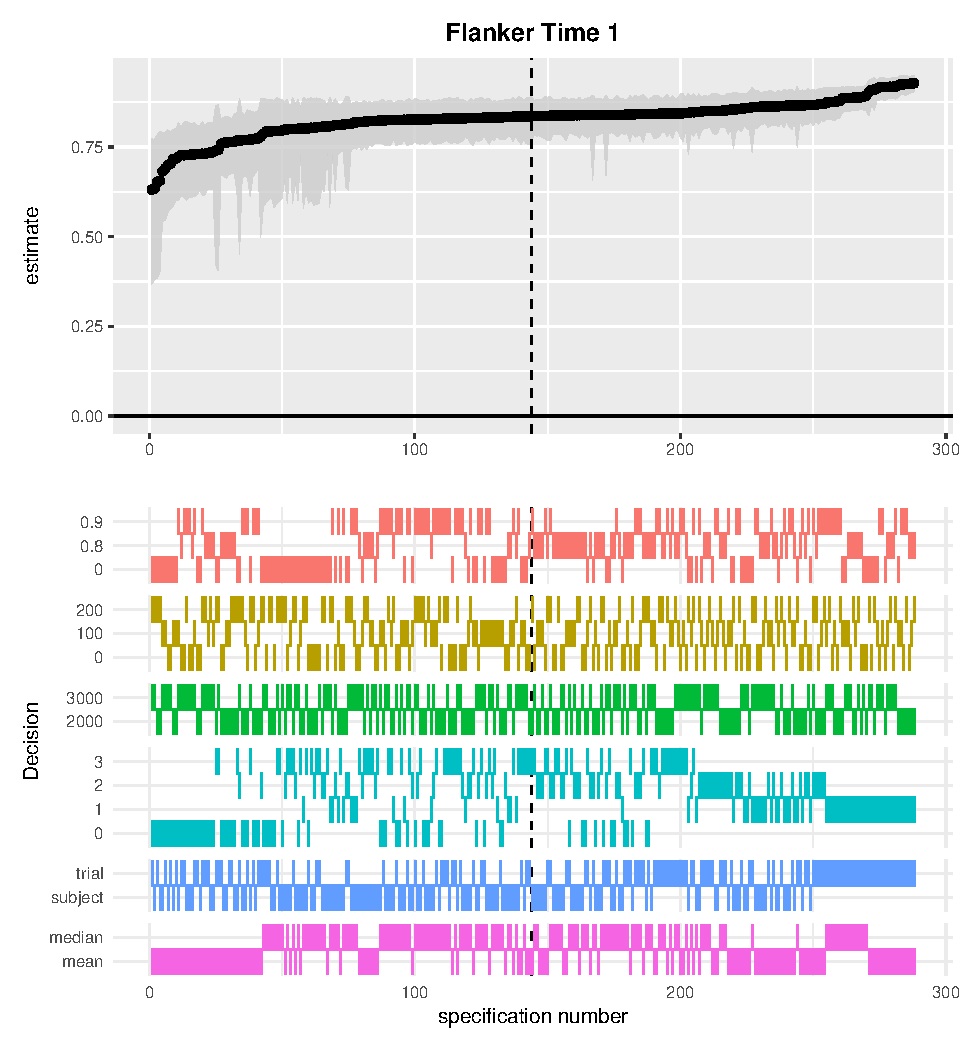
\includegraphics{Reliability_Multiverse_files/figure-latex/unnamed-chunk-8-1.pdf}
\caption{\label{fig:unnamed-chunk-8}Internal consistency reliability multiverse for Flanker RT cost at time 1}
\end{figure}

\newpage

\hypertarget{flanker-time-2-internal-consistency}{%
\subsubsection{Flanker Time 2: Internal Consistency}\label{flanker-time-2-internal-consistency}}

The median reliability estimate was 0.74, 95\% CI {[}0.63,0.88{]}. Estimates ranged from 0.59 to 0.90. 66\% of the reliability estimates were \textgreater{} 0.7.

\begin{figure}
\centering
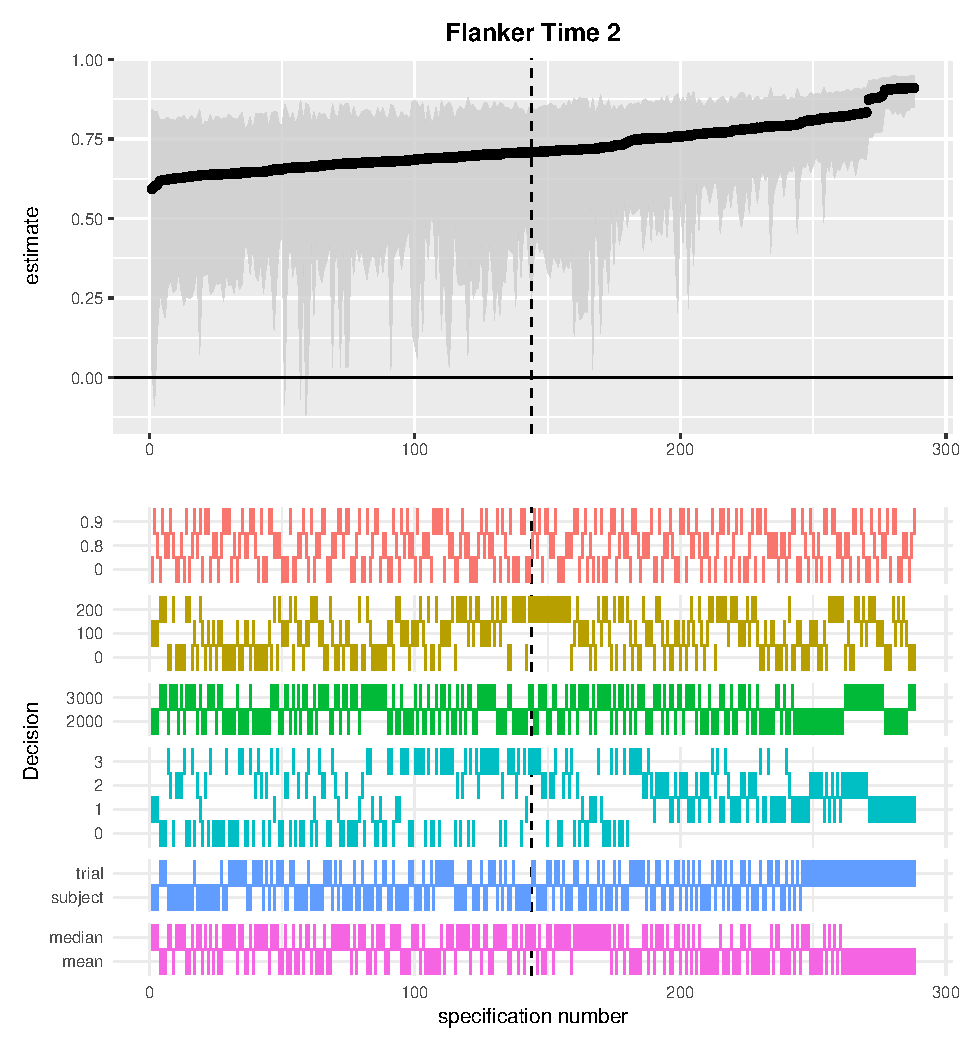
\includegraphics{Reliability_Multiverse_files/figure-latex/unnamed-chunk-9-1.pdf}
\caption{\label{fig:unnamed-chunk-9}Internal consistency reliability multiverse for Flanker RT cost at time 2}
\end{figure}

\newpage

\hypertarget{flanker-test-retest}{%
\subsubsection{Flanker: test-retest}\label{flanker-test-retest}}

The median reliability estimate was 0.55, 95\% CI {[}0.30,0.69{]}. Estimates ranged from 0.28 to 0.72. 2\% of the reliability estimates were \textgreater{} 0.7.

\begin{figure}
\centering
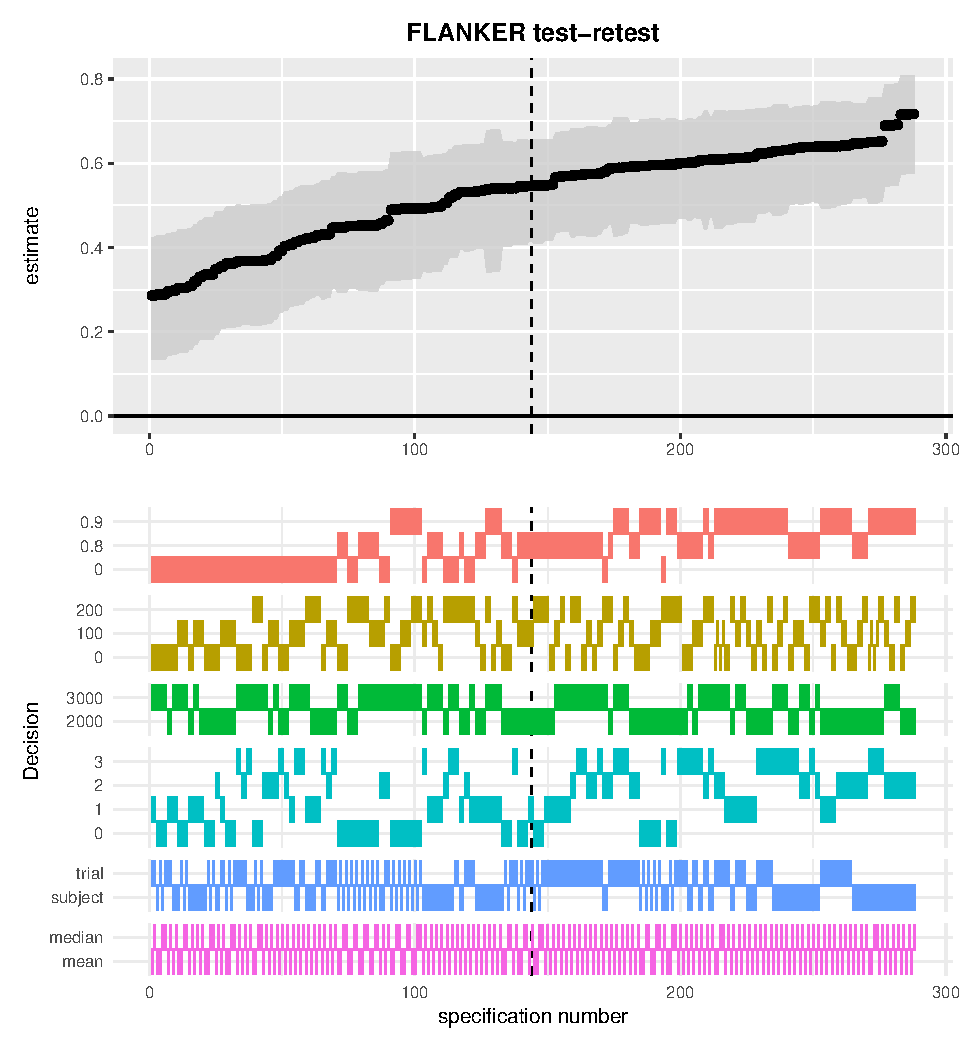
\includegraphics{Reliability_Multiverse_files/figure-latex/unnamed-chunk-10-1.pdf}
\caption{\label{fig:unnamed-chunk-10}Test-retest reliability multiverse for Flanker RT cost}
\end{figure}

\newpage

\hypertarget{overlapping-time-1-and-time-2-multiverses}{%
\subsubsection{Overlapping time 1 and time 2 multiverses}\label{overlapping-time-1-and-time-2-multiverses}}

In the final two figures I overlap the time 1 and time 2 multiverses, separately for the Stroop and Flanker data. The specifications are ordered by the reliability estimates at time 1 for each measure (Figures 1 and 3). These figures allow us to compare the patterns of reliability estimates following the same data processing decisions.

\begin{figure}
\centering
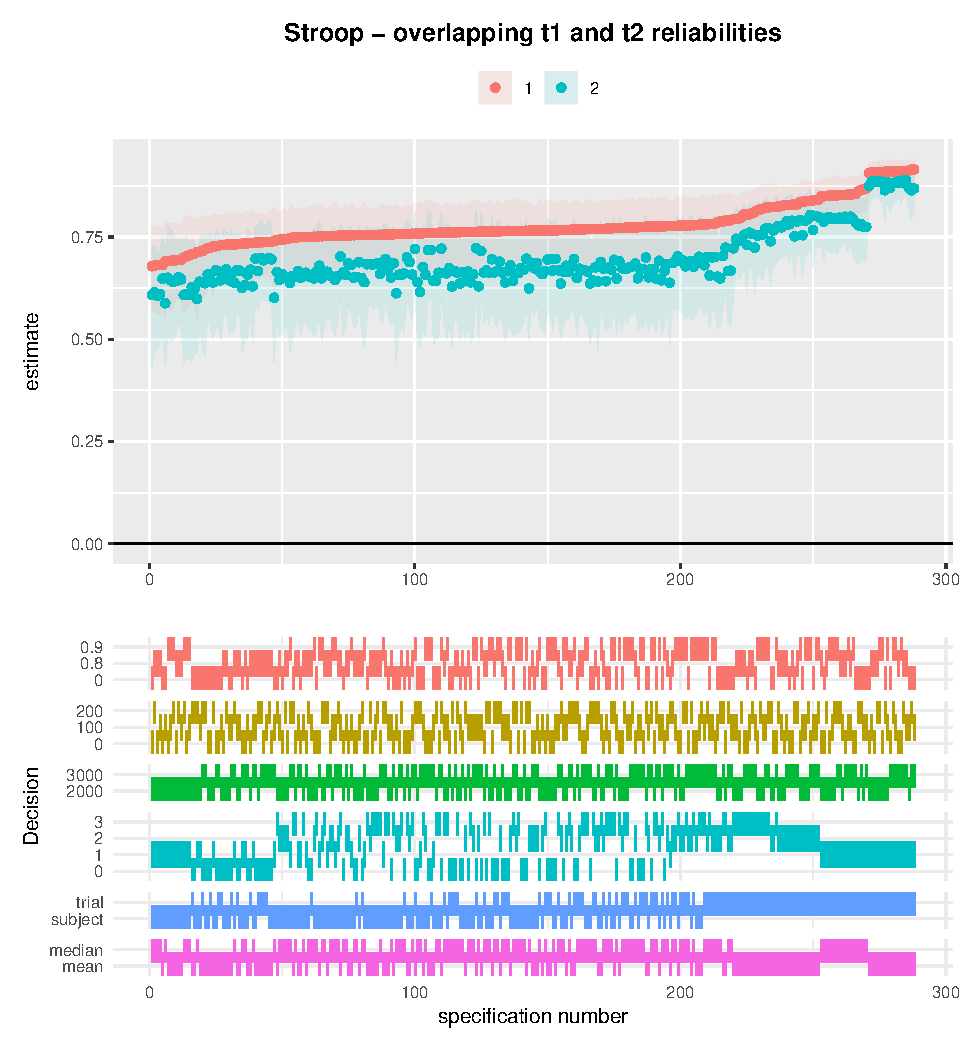
\includegraphics{Reliability_Multiverse_files/figure-latex/unnamed-chunk-11-1.pdf}
\caption{\label{fig:unnamed-chunk-11}Overlapped internal consistency reliability multiverse for Stroop RT cost at times 1 and 2}
\end{figure}

\begin{figure}
\centering
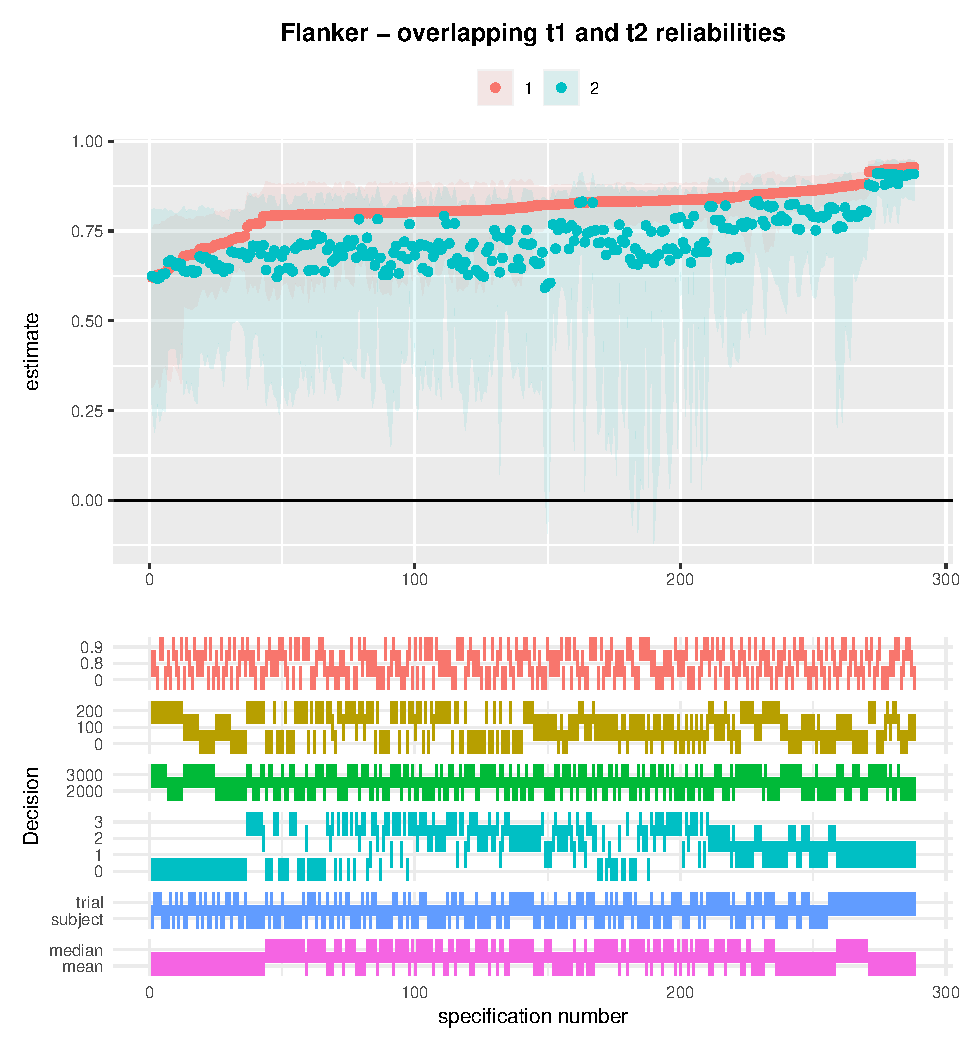
\includegraphics{Reliability_Multiverse_files/figure-latex/unnamed-chunk-12-1.pdf}
\caption{\label{fig:unnamed-chunk-12}Overlapped internal consistency reliability multiverse for Flanker RT cost at times 1 and 2}
\end{figure}

\hypertarget{discussion}{%
\section{Discussion}\label{discussion}}

In the results section I presented visualisations of six multiverse analyses and an additional two visualisations overlapping the internal consistency multiverses. The range of reliability estimates was 0.24-0.31 for internal consistency and 0.16-0.43 for test-retest. In the introduction, I reminded the reader that reliability estimates are a product of the sample and the population they are drawn from, the task (including any differences in implementation), and the circumstances in which the measurement was obtained; i.e.~reliability is not an inherent quality of the task itself. The first conclusion to take from these multiverse analyses is that data processing specifications are also an integral part of this list.

At the onset of this project, I thought it reasonable to assume that a particular feature of the data processing path might result in consistently higher (and lower) reliability estimates. The clearest indication we can take from these analyses is that there is no single set of data processing specifications, or combination of data processing decisions, that lead to improved reliability. The wide ranges of estimates are an additional cause for concern. Seemingly arbitrary data processing decisions can lead to differences of more than .3 in the reliability of a measure. These decisions are equally reasonable and logical choices, and we should not expect them to have meaningful impact on the theoretical questions being asked of the data. The reliability multiverse analyses presented here demonstrate this using data from a Stroop and a Flanker task. As well as across tasks, overlapping the time 1 and time 2 multiverses for both tasks highlights that even the same set of specifications does not lead to directly comparable internal consistency reliability estimates over time. data processing decisions appear to be extremely important contributors to measure reliability, but their influence is unpredictable and arbitrary.

Despite this pessimistic outlook, there is a trend across the multiverse analyses that inspires some small hope. There is a trend for increased reliability in specifications that exclude trials based on a standard deviation cutoff away from the trial mean RT, rather than away from the participant's grand average RT. The highest reliability estimates are also where a relative RT cut-off of one standard deviation from the mean is used. However, I have yet to read a paper that used such a conservative approach to removing outlier trials (approximately 30\% of trials). I am not convinced that these small trends offer strong insight into how we should process task data to maximise reliability; further exploration is undoubtedly needed. In the core of this discussion I raise several open questions and suggest some plausible actions that could be taken to mitigate some of the risk reliability heterogeneity poses.

\hypertarget{how-do-we-guard-against-reliability-heterogeneity}{%
\subsection{How do we guard against reliability heterogeneity?}\label{how-do-we-guard-against-reliability-heterogeneity}}

Low reliability attenuates effect sizes estimated from tests in which the measure is used. It is therefore important to take reliability heterogeneity into account when comparing effect sizes (for several clear examples, see Cooper, Gonthier, Barch, \& Braver, 2017). It is plausible that some studies may have obtained smaller or larger effect sizes than others based, in part, on the reliability of the measurements taken. Similarly, identical observed effect sizes may represent very different \enquote{true} effect sizes, if reliability is taken into account. Recently, Wiernik and Dahlke (2020) made a strong case for correcting for measurement error in meta-analyses, and provide the necessary formula and code for doing so. There are several actions we can take to begin to account for reliability heterogeneity.

\hypertarget{two-simple-recommendations.}{%
\subsubsection{Two simple recommendations.}\label{two-simple-recommendations.}}

To briefly reiterate two recommendations I and my colleagues have made previously: report all data processing steps taken, and report the reliability of measures analysed (Parsons et al., 2019). These recommendations will not \enquote{fix} potential psychometric issues within one's study, or reliability heterogeniety across studies. However, complete reporting of data processing will assist in the computational reproducibility of one's results. Reporting psychometric information will assist in the interpretation of results, including comparisons of effect sizes, as well as provide useful information about the utility of a task in studies of individual differences.

\hypertarget{adopt-a-modelling-approach.}{%
\subsubsection{Adopt a modelling approach.}\label{adopt-a-modelling-approach.}}

Incorporating trial level variation into our analyses with hierarchical modelling approaches will likely be a vital step in protecting us against reliability heterogeneity. Psychological effects are often heterogeneous across individuals (Bolger, Zee, Rossignac-Milon, \& Hassin, 2019), and factors within tasks have important effects (e.g.~stimuli differences; DeBruine \& Barr, 2019). It follows that our models should take trial-level variation into account. Using the Stroop and Flanker data from Hedge et al.~(2018) Rouder, Kumar, and Haaf (2019; also see Rouder \& Haaf, 2018) demonstrated that hierarchical models should be used to account for error in measurement (for additional guidance on applying this modelling, see Haines, 2019). Adopting this approach would have the benefit of \enquote{correcting} the effect size estimate (and standard error) for measurement error as part of the model. Rouder and colleagues demonstrate that this is also a more effective approach than \enquote{correcting} the effect size estimate using e.g.~Spearman's correction for attenuation formula (Spearman, 1904). Yet, even better corrections cannot fully save us from measurement error.

The benefits of adopting multilevel approaches could be demonstrated empirically with an extension of the multiverse approach adopted here. If we were to extract outcome data from the multiverse and correlate it with another variable (held constant across the multiverses), we would expect the correlation effect size to increase with increased reliability estimates. I expect that incorporating hierarchical modelling into the multiverse would lead to reduced heterogeneity across the effect size estimates as error has been accounted for in the model. Though, we should expect the confidence interval around the estimate to reduce in size with increasing reliability -- reducing error is almost always a good thing. I believe this would be a strong argument for more widespread use of hierarchical models in the analysis of behavioural measures.

\hypertarget{limitations-and-room-for-expansion}{%
\subsection{Limitations and room for expansion}\label{limitations-and-room-for-expansion}}

One potential limitation of this study is the focus on only two tasks. It is possible that data from other tasks tend to yield more or less consistent patterns of reliability estimates across data processing specifications. Similarly, I have only examined RT costs (i.e.~a difference score between two trial types) as the outcome measure. The analyses could have examined accuracy rates, RT averages, signal detection, and a wide variety of outcome measures. It is very possible that other outcome indices would be more or less consistently reliable across the range of data processing specifications. I opted for brevity in this paper by selecting only two tasks from Hedge et al.~(2018) and looked at only RT costs as the outcome; I welcome future work seeking to examine a wider range of tasks and outcome indices.

There is a paradox in measurement reliability (see 2018): Experimental effects that are highly replicable (for example, the Stroop effect) may also show low reliability. Homogeneity within groups or experimental conditions allows for larger and more robust effects; researchers can opt to develop tasks that capitalise on homogeneity. Unfortunately, reliability requires robust individual differences (and vice versa). Highly reliable measures by necessity show consistent, potentially large, individual differences and would not be suitable for group differences or experimental research.

As a result, measures tend to be more appropriate for questions of a) assessing differences between groups or experimental conditions, or b) correlational or individual differences. I was primarily concerned with the use of these measures in individual differences research - hence the focus on reliability. Yet, it would be overly simplistic to assert that the discussions in this paper do not also relate to experimental differences questions. Indeed, the data processing specifications that maximise the measure's utility in individual differences analyses will also hinder the measure's utility in experimental quesitons. Further research would be needed to quantify the relative influences on correlational vs experimental analyses. Yet, large fluctuations in relative between-subjects vs within-subjects variance, due to data processing, holds importance for any research question.

\hypertarget{what-about-validity}{%
\subsection{What about validity?}\label{what-about-validity}}

Others have previously demonstrated that measures are often used ad hoc or with little reported validation efforts (e.g.~Flake et al., 2017; Hussey \& Hughes, 2018). This study cannot begin to assess the influence of data processing flexibility on measure validity -- nor did this paper attempt to address this question. Reliability is only one piece of evidence needed to demonstrate the validity of a measure. Yet, it is an important piece of evidence as \enquote{reliability provides an upper bound for validity} (Zuo, Xu, \& Milham, 2019, p. 3). While we cannot directly conclude that flexibility in data processing influences measure validity, we should look to further research to investigate. One possibility would be to conduct a validity multiverse analysis similar to the \enquote{Many Analysts, One Data Set} project (Silberzahn et al., 2018). In this project, 29 teams (61 analysts total) analysed the same dataset. The teams adopted a number of different analytic approaches which resulted in a range of results. The authors concluded that, \enquote{Uncertainty in interpreting research results is therefore not just a function of statistical power or the use of questionable research practices; it is also a function of the many reasonable decisions that researchers must make in order to conduct the research} (page 354).

\hypertarget{returning-to-the-garden}{%
\subsection{Returning to the garden}\label{returning-to-the-garden}}

My intention for this project was to provide some indication about the influence of data processing pathways on the reliability of our cognitive measurements. The influence can be profound; the multiverse analyses show large differences between the highest and lowest reliability estimates. Yet, we see little consistency in the pattern of decisions leading to higher, or lower, estimates. We have the worst of both worlds: data processing decisions are largely arbitrary, yet can have a large -- relatively unpredictable -- impact on the resulting reliability estimates. Briefly returning to the garden of forking paths metaphor; I imagined that this project would help illuminate the point in which our hypothetical researcher would enter the garden, based on their data processing decisions. But, our investigation has uncovered an unfortunate secret: Our researcher's forking paths are almost entirely arbitrary and interwoven. Each path diverges wildly, leading to almost anywhere in the garden. It is as if our researcher is simply spinning in dizzy circles until they stumble somewhere along the fence of reliability. I discussed several actions researchers can take collectively to help with the issue. But, by no means were these remedies to our reliability issues, nor would they directly help issues with the validity of our measurements.

I am concerned that we sit on the precipice of a measurement crisis. The so-called replication crisis shook much of our field into widespread and ongoing reforms. Yet, much of the focus has been on improving methodological and statistical practices. This is undoubtedly worthwhile, but largely omits discussion of reliability and validity of our measurements -- despite our measurements forming the basis of any outcome or inference. This oversight feels like repairing a damaged wall at the same time as ignoring the shifting foundations under it. I hope that this paper, and similar work, highlights the issue and encourages researchers to place more emphasis on quality measurement. As a field, we can orchestrate a measurement revolution (cf.~the ``credibility revolution'', Vazire, 2018) in which the quality and validity of our measurements is placed an order of importance above obtaining desired results. If the reader takes home a single message from this paper, let it be \enquote{measurement matters}.

\newpage

\hypertarget{references}{%
\section{References}\label{references}}

\begingroup
\setlength{\parindent}{-0.5in}
\setlength{\leftskip}{0.5in}

\hypertarget{refs}{}
\leavevmode\hypertarget{ref-R-gridExtra}{}%
Auguie, B. (2017). \emph{GridExtra: Miscellaneous functions for "grid" graphics}. Retrieved from \url{https://CRAN.R-project.org/package=gridExtra}

\leavevmode\hypertarget{ref-R-papaja}{}%
Aust, F., \& Barth, M. (2020). \emph{papaja: Create APA manuscripts with R Markdown}. Retrieved from \url{https://github.com/crsh/papaja}

\leavevmode\hypertarget{ref-bolger_causal_2019}{}%
Bolger, N., Zee, K. S., Rossignac-Milon, M., \& Hassin, R. R. (2019). Causal processes in psychology are heterogeneous. \emph{Journal of Experimental Psychology: General}, \emph{148}(4), 601--618. \url{https://doi.org/10.1037/xge0000558}

\leavevmode\hypertarget{ref-cooper_role_2017}{}%
Cooper, S. R., Gonthier, C., Barch, D. M., \& Braver, T. S. (2017). The role of psychometrics in individual differences research in cognition: A case study of the AX-CPT. \emph{Frontiers in Psychology}, \emph{8}, 1--16. \url{https://doi.org/10.3389/fpsyg.2017.01482}

\leavevmode\hypertarget{ref-debruine_understanding_2019}{}%
DeBruine, L. M., \& Barr, D. J. (2019). \emph{Understanding mixed effects models through data simulation} (preprint). PsyArXiv. \url{https://doi.org/10.31234/osf.io/xp5cy}

\leavevmode\hypertarget{ref-flake_measurement_2019}{}%
Flake, J. K., \& Fried, E. I. (2019). \emph{Measurement Schmeasurement: Questionable Measurement Practices and How to Avoid Them} (preprint). PsyArXiv. \url{https://doi.org/10.31234/osf.io/hs7wm}

\leavevmode\hypertarget{ref-flake_construct_2017}{}%
Flake, J. K., Pek, J., \& Hehman, E. (2017). Construct Validation in Social and Personality Research: Current Practice and Recommendations. \emph{Social Psychological and Personality Science}, \emph{8}(4), 370--378. \url{https://doi.org/10.1177/1948550617693063}

\leavevmode\hypertarget{ref-fried_measurement_2018}{}%
Fried, E. I., \& Flake, J. K. (2018). Measurement matters. \emph{Observer}. Retrieved from \url{https://www.psychologicalscience.org/observer/measurement-matters}

\leavevmode\hypertarget{ref-gawronski_response_2011-1}{}%
Gawronski, B., Deutsch, R., \& Banse, R. (2011). Response interference tasks as indirect measures of automatic associations. In \emph{Cognitive methods in social psychology.} (pp. 78--123). New York, NY, US: The Guilford Press.

\leavevmode\hypertarget{ref-gelman_garden_2013}{}%
Gelman, A., \& Loken, E. (2013). The garden of forking paths: Why multiple comparisons can be a problem, even when there is no ``fishing expedition'' or ``p-hacking'' and the research hypothesis was posited ahead of time, 17. Retrieved from \url{https://doi.org/dx.doi.org/10.1037/a0037714}

\leavevmode\hypertarget{ref-haines_thinking_2019}{}%
Haines, N. (2019). Thinking generatively: Why do we use atheoretical statistical models to test substantive psychological theories? Retrieved from \url{http://haines-lab.com/post/thinking-generatively-why-do-we-use-atheoretical-statistical-models-to-test-substantive-psychological-theories/}

\leavevmode\hypertarget{ref-hedge_reliability_2018}{}%
Hedge, C., Powell, G., \& Sumner, P. (2018). The reliability paradox: Why robust cognitive tasks do not produce reliable individual differences. \emph{Behavior Research Methods}, \emph{50}(3), 1166--1186. \url{https://doi.org/10.3758/s13428-017-0935-1}

\leavevmode\hypertarget{ref-R-purrr}{}%
Henry, L., \& Wickham, H. (2019). \emph{Purrr: Functional programming tools}. Retrieved from \url{https://CRAN.R-project.org/package=purrr}

\leavevmode\hypertarget{ref-hussey_hidden_2018}{}%
Hussey, I., \& Hughes, S. (2018). Hidden invalidity among fifteen commonly used measures in social and personality psychology. \url{https://doi.org/10.31234/osf.io/7rbfp}

\leavevmode\hypertarget{ref-jones_failed_2018-1}{}%
Jones, A., Christiansen, P., \& Field, M. (2018). Failed attempts to improve the reliability of the alcohol visual probe task following empirical recommendations. \emph{Psychology of Addictive Behaviors}, \emph{32}(8), 922--932. \url{https://doi.org/10.1037/adb0000414}

\leavevmode\hypertarget{ref-lakens_justify_2018}{}%
Lakens, D., Adolfi, F. G., Albers, C. J., Anvari, F., Apps, M. A. J., Argamon, S. E., \ldots{} Zwaan, R. A. (2018). Justify your alpha. \emph{Nature Human Behaviour}, \emph{2}(3), 168--171. \url{https://doi.org/10.1038/s41562-018-0311-x}

\leavevmode\hypertarget{ref-leek_p_2015}{}%
Leek, J. T., \& Peng, R. D. (2015). P values are just the tip of the iceberg. \emph{Nature}, \emph{520}, 612. \url{https://doi.org/10.1038/520612a}

\leavevmode\hypertarget{ref-loken_measurement_2017}{}%
Loken, E., \& Gelman, A. (2017). Measurement error and the replication crisis. \emph{Science}, \emph{355}(6325), 584--585. \url{https://doi.org/10.1126/science.aal3618}

\leavevmode\hypertarget{ref-R-tibble}{}%
Müller, K., \& Wickham, H. (2019). \emph{Tibble: Simple data frames}. Retrieved from \url{https://CRAN.R-project.org/package=tibble}

\leavevmode\hypertarget{ref-orben_association_2019}{}%
Orben, A., \& Przybylski, A. K. (2019). The association between adolescent well-being and digital technology use. \emph{Nature Human Behaviour}, \emph{3}(2), 173--182. \url{https://doi.org/10.1038/s41562-018-0506-1}

\leavevmode\hypertarget{ref-parsons_splithalf:_2019}{}%
Parsons, S. (2019). \emph{Splithalf: Robust estimates of split half reliability}. Retrieved from \url{https://doi.org/10.6084/m9.figshare.5559175.v5}

\leavevmode\hypertarget{ref-R-splithalf}{}%
Parsons, S. (2020). Splithalf; robust estimates of split half reliability. Retrieved from \url{https://doi.org/10.6084/m9.figshare.5559175.v5}

\leavevmode\hypertarget{ref-parsons_psychological_2019}{}%
Parsons, S., Kruijt, A.-W., \& Fox, E. (2019). Psychological Science Needs a Standard Practice of Reporting the Reliability of Cognitive-Behavioral Measurements. \emph{Advances in Methods and Practices in Psychological Science}, \emph{2}(4), 378--395. \url{https://doi.org/10.1177/2515245919879695}

\leavevmode\hypertarget{ref-R-patchwork}{}%
Pedersen, T. L. (2019). \emph{Patchwork: The composer of plots}. Retrieved from \url{https://CRAN.R-project.org/package=patchwork}

\leavevmode\hypertarget{ref-price_empirical_2015}{}%
Price, R. B., Kuckertz, J. M., Siegle, G. J., Ladouceur, C. D., Silk, J. S., Ryan, N. D., \ldots{} Amir, N. (2015). Empirical recommendations for improving the stability of the dot-probe task in clinical research. \emph{Psychological Assessment}, \emph{27}(2), 365--376. \url{https://doi.org/10.1037/pas0000036}

\leavevmode\hypertarget{ref-quintana_gps_2019}{}%
Quintana, D. S., \& Heathers, J. (2019). A GPS in the Garden of Forking Paths (with Amy Orben). Retrieved from \url{10.17605/OSF.IO/38KPE}

\leavevmode\hypertarget{ref-R-base}{}%
R Core Team. (2018). \emph{R: A language and environment for statistical computing}. Vienna, Austria: R Foundation for Statistical Computing. Retrieved from \url{https://www.R-project.org/}

\leavevmode\hypertarget{ref-revelle_psych:_2017-1}{}%
Revelle, W. (2017). \emph{Psych: Procedures for Personality and Psychological Research}. Northwestern University, Evanston, Illinois, USA.

\leavevmode\hypertarget{ref-R-psych}{}%
Revelle, W. (2019). \emph{Psych: Procedures for psychological, psychometric, and personality research}. Evanston, Illinois: Northwestern University. Retrieved from \url{https://CRAN.R-project.org/package=psych}

\leavevmode\hypertarget{ref-rohrer_probing_2017}{}%
Rohrer, J. M., Egloff, B., \& Schmukle, S. C. (2017). Probing Birth-Order Effects on Narrow Traits Using Specification-Curve Analysis. \emph{Psychological Science}, \emph{28}(12), 1821--1832. \url{https://doi.org/10.1177/0956797617723726}

\leavevmode\hypertarget{ref-rouder_psychometrics_2018}{}%
Rouder, J., \& Haaf, J. M. (2018). A Psychometrics of Individual Differences in Experimental Tasks. \url{https://doi.org/10.31234/osf.io/f3h2k}

\leavevmode\hypertarget{ref-rouder_why_2019}{}%
Rouder, J., Kumar, A., \& Haaf, J. M. (2019). Why Most Studies of Individual Differences With Inhibition Tasks Are Bound To Fail. \url{https://doi.org/10.31234/osf.io/3cjr5}

\leavevmode\hypertarget{ref-schmukle_unreliability_2005}{}%
Schmukle, S. C. (2005). Unreliability of the dot probe task. \emph{European Journal of Personality}, \emph{19}(7), 595--605. \url{https://doi.org/10.1002/per.554}

\leavevmode\hypertarget{ref-silberzahn_many_2018}{}%
Silberzahn, R., Uhlmann, E. L., Martin, D. P., Anselmi, P., Aust, F., Awtrey, E., \ldots{} Nosek, B. A. (2018). Many Analysts, One Data Set: Making Transparent How Variations in Analytic Choices Affect Results. \emph{Advances in Methods and Practices in Psychological Science}, \emph{1}(3), 337--356. \url{https://doi.org/10.1177/2515245917747646}

\leavevmode\hypertarget{ref-simmons_false-positive_2011}{}%
Simmons, J. P., Nelson, L. D., \& Simonsohn, U. (2011). False-Positive Psychology: Undisclosed Flexibility in Data Collection and Analysis Allows Presenting Anything as Significant. \emph{Psychological Science}, \emph{22}(11), 1359--1366. \url{https://doi.org/10.1177/0956797611417632}

\leavevmode\hypertarget{ref-simonsohn_specification_2015}{}%
Simonsohn, U., Simmons, J. P., \& Nelson, L. D. (2015). Specification Curve: Descriptive and Inferential Statistics on All Reasonable Specifications. \emph{SSRN Electronic Journal}. \url{https://doi.org/10.2139/ssrn.2694998}

\leavevmode\hypertarget{ref-spearman_proof_1904}{}%
Spearman, C. (1904). The Proof and Measurement of Association between Two Things. \emph{The American Journal of Psychology}, \emph{15}(1), 72. \url{https://doi.org/10.2307/1412159}

\leavevmode\hypertarget{ref-staugaard_reliability_2009}{}%
Staugaard, S. R. (2009). Reliability of two versions of the dot-probe task using photographic faces. \emph{Psychology Science Quarterly}, \emph{51}(3), 339--350.

\leavevmode\hypertarget{ref-steegen_increasing_2016}{}%
Steegen, S., Tuerlinckx, F., Gelman, A., \& Vanpaemel, W. (2016). Increasing Transparency Through a Multiverse Analysis. \emph{Perspectives on Psychological Science}, \emph{11}(5), 702--712. \url{https://doi.org/10.1177/1745691616658637}

\leavevmode\hypertarget{ref-R-Cairo}{}%
Urbanek, S., \& Horner, J. (2019). \emph{Cairo: R graphics device using cairo graphics library for creating high-quality bitmap (png, jpeg, tiff), vector (pdf, svg, postscript) and display (x11 and win32) output}. Retrieved from \url{https://CRAN.R-project.org/package=Cairo}

\leavevmode\hypertarget{ref-vazire_implications_2018}{}%
Vazire, S. (2018). Implications of the Credibility Revolution for Productivity, Creativity, and Progress. \emph{Perspectives on Psychological Science}, \emph{13}(4), 411--417. \url{https://doi.org/https://doi.org/10.1177/1745691617751884}

\leavevmode\hypertarget{ref-R-ggplot2}{}%
Wickham, H. (2016). \emph{Ggplot2: Elegant graphics for data analysis}. Springer-Verlag New York. Retrieved from \url{https://ggplot2.tidyverse.org}

\leavevmode\hypertarget{ref-R-forcats}{}%
Wickham, H. (2019a). \emph{Forcats: Tools for working with categorical variables (factors)}. Retrieved from \url{https://CRAN.R-project.org/package=forcats}

\leavevmode\hypertarget{ref-R-stringr}{}%
Wickham, H. (2019b). \emph{Stringr: Simple, consistent wrappers for common string operations}. Retrieved from \url{https://CRAN.R-project.org/package=stringr}

\leavevmode\hypertarget{ref-R-tidyverse}{}%
Wickham, H., Averick, M., Bryan, J., Chang, W., McGowan, L. D., François, R., \ldots{} Yutani, H. (2019). Welcome to the tidyverse. \emph{Journal of Open Source Software}, \emph{4}(43), 1686. \url{https://doi.org/10.21105/joss.01686}

\leavevmode\hypertarget{ref-R-dplyr}{}%
Wickham, H., François, R., Henry, L., \& Müller, K. (2019). \emph{Dplyr: A grammar of data manipulation}. Retrieved from \url{https://CRAN.R-project.org/package=dplyr}

\leavevmode\hypertarget{ref-R-tidyr}{}%
Wickham, H., \& Henry, L. (2019). \emph{Tidyr: Tidy messy data}. Retrieved from \url{https://CRAN.R-project.org/package=tidyr}

\leavevmode\hypertarget{ref-R-readr}{}%
Wickham, H., Hester, J., \& Francois, R. (2018). \emph{Readr: Read rectangular text data}. Retrieved from \url{https://CRAN.R-project.org/package=readr}

\leavevmode\hypertarget{ref-wiernik_obtaining_2020}{}%
Wiernik, B. M., \& Dahlke, J. A. (2020). Obtaining Unbiased Results in Meta-Analysis: The Importance of Correcting for Statistical Artifacts. \emph{Advances in Methods and Practices in Psychological Science}. \url{https://doi.org/10.1177/2515245919885611}

\leavevmode\hypertarget{ref-zuo_harnessing_2019}{}%
Zuo, X.-N., Xu, T., \& Milham, M. P. (2019). Harnessing reliability for neuroscience research. \emph{Nature Human Behaviour}. \url{https://doi.org/10.1038/s41562-019-0655-x}

\endgroup

\end{document}
